\section{Results}

\begin{figure}[t]
  \centering
  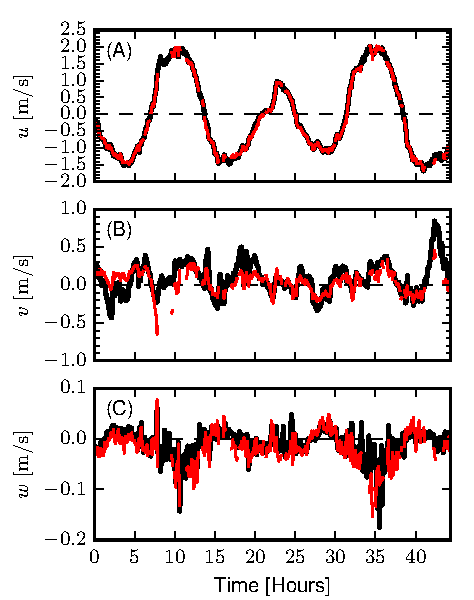
\includegraphics{TimeFig02}
  \caption{Time series of tidal velocity at Admiralty Head from TTM measurements (black), and an acoustic Doppler profiler (red). The profiler measurements--taken at the same depth as the ADV on the TTM---were contaminated by acoustic reflection from the strongback fin when it was inline with one of the profiler's beams. Note that the vertical scale on the three axes vary by more than an order of magnitude; the small ticks in A and B are equivalent to the ticks in C.}
  \label{fig:vel_time}
\end{figure}

\subsection{Mean velocity}

A comparison of mean velocity measured by an ADV-IMU mounted on a TTM, to that of an upward-looking acoustic Doppler profiler mounted on the TTM anchor is presented in Figure \ref{fig:vel_time}. This shows excellent agreement between the ADV and Doppler profiler measurements of velocity. The $u$, $v$ and $w$ components have a root-mean-square error of 0.05, 0.13 and 0.03 m/s, respectively. While it is important to note that their is some discrepancy between ADP and ADV measured velocities (especially in the $v$-component, which is most likely due to incomplete motion correction), the agreement between the magnitude and direction of these independent velocity measurements indicates that moored ADV-IMUs provide a reliable estimate of velocity in the Earth's reference frame.

\subsection{TTM Spectra}

\begin{figure*}[t]
  \centering
  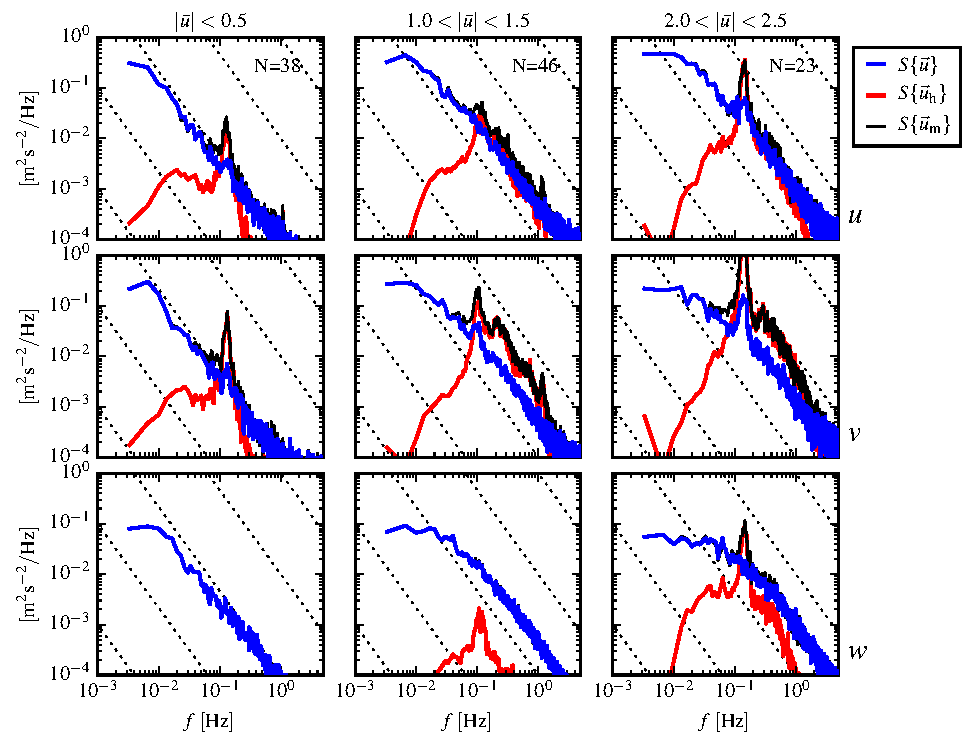
\includegraphics{SpecFig02_TTM02B-top}
  \caption{Turbulence spectra from the TTM for 3 ranges of mean stream-wise velocity (first column: $|u|< 0.5$ m/s, second column: $1 < |u| < 1.5$ m/s, third column: $2 < |u| < 2.5$ m/s). The rows are for each component of velocity (top: $u$, middle: $v$, bottom: $w$). The uncorrected spectra are in black and the corrected spectra are blue. The spectra of ADV head motion, $\uhead$, is red. Diagonal dotted-lines indicate a $f^{-5/3}$ slope. N is the number of spectral-ensembles in each column.}
  \label{fig:spec:ttm}
\end{figure*}

As discussed in detail in the companion paper, the mooring motion of the TTM, $\spec{\uhead}$, has a peak at 0.1 to 0.2 Hz from swaying of the mooring that is most likely driven by eddy-shedding from the spherical buoy (Figure \ref{fig:spec:ttm}, red lines). There is also broad-band motion that is associated with fluttering of the strongback fin around the mooring line. Both of these motions are especially energetic in the $v$-component spectra, because this is the direction in-which the TTM mooring system is most unstable. As is expected from fluid-structure interaction theory the amplitude of these motions increases with increasing mean velocity \cite[]{Morison++1950}.

The mooring motion contaminates the uncorrected ADV-measurements of velocity, \spec{\umeas}, whenever the amplitude of the motion is similar to or greater than the amplitude of the turbulence. Fortunately, much of this motion can be removed using the IMU's motion signals as detailed in section \ref{sec:methods}. Lacking an independent measurement of turbulence velocity at this site, we interpret the agreement of these spectra with turbulence theory as evidence of the success of the method. In particular, for each mean-flow speed the spectra decay with a $f^{-5/3}$ slope and have equal amplitude across the velocity components. These results are consistent with Kolmogorov's (1941) theory of isotropic turbulence, and are consistent with other measurements of turbulence in energetic tidal channels from stationary platforms \citep[]{Kolmogorov1941c,Walter++2011,Thomson++2012,McMillan++2016}.

As successful as motion correction is, some of the motion contamination persists in $\spec{\ue}$. This is most notable in the $v$-component spectra at the highest flow speeds where a peak in $\spec{v}$ at 0.15 Hz is nearly an order of magnitude larger than a typical turbulence spectral fit to the other frequencies would indicate. This persistent motion contamination is evident to a lesser degree in the $u$-component spectra at the highest flow speed, and in the $v$-component spectra at lower flow speeds.  The $w$-component spectra appear to have no persistent motion contamination. This is largely because the amplitude of the motion in this direction is much lower than for the other two components. In fact, for these measurements, the $w$-component of mooring motion is so low that $w$-component motion correction is significant only at the highest flow speeds (i.e. motion correction removes the 0.15 Hz peak).

The amplitude of the persistent motion contamination peaks at 0.15 Hz are a factor of 5 to 10 times smaller than the amplitude of the ADV head motion itself. This suggests the Microstrain IMU's motion signals can be used to effectively correct for mooring motion at 0.15 Hz when the amplitude of that motion is less than 5 times the amplitude of the real turbulence spectrum.

% Does this belong in the discussion?
This reveals an ancillary benefit of the IMU measurements, which is that they can assist with identifying and accounting for persistent sources of motion contamination. For example, one of the most common uses of turbulence spectra is for the calculation of the turbulent kinetic energy dissipation rate, $\epsilon$, or for calculating the total turbulent kinetic energy, $\tke$. In particular, the regions of the spectrum where the motion is a factor of 3 to 5 larger than the measured signal can be excluded from a spectral fit. The fit can then be used to estimate $\tke$ and $\epsilon$. 
% Do we need to say something about the $v$-component time series being contaminated, but the $w$ and $u$ are relatively clean?

\subsection{StableMoor Spectra}

The spectra of the stablemoor motion has a broader peak with a maximum amplitude that is at approximately half the frequency of the TTM spectral peak (Figure \ref{fig:spec:sm}). The motion of this platform also does not have high-frequency `sub-peaks' or other high-frequency broad-banded excitation. These characteristics of the motion are most-likely due to the more massive and hydro-dynamically streamlined nature of the platform. 

Like the TTM, the motion-corrected spectra from the StableMoor are consistent with turbulence theory and previous observations. Most importantly, there is an improvement in the quality of the motion corrected spectra compared to the TTM. In particular their does not appear to be significant persistent motion contamination peaks in these spectra. When the assumption that $\ulow=0$ is made, peaks and troughs are seen in the data, which suggests that the improvement in motion correction is largely the result of an accurate measurement of $\ulow$.

\begin{figure*}[t]
  \centering
  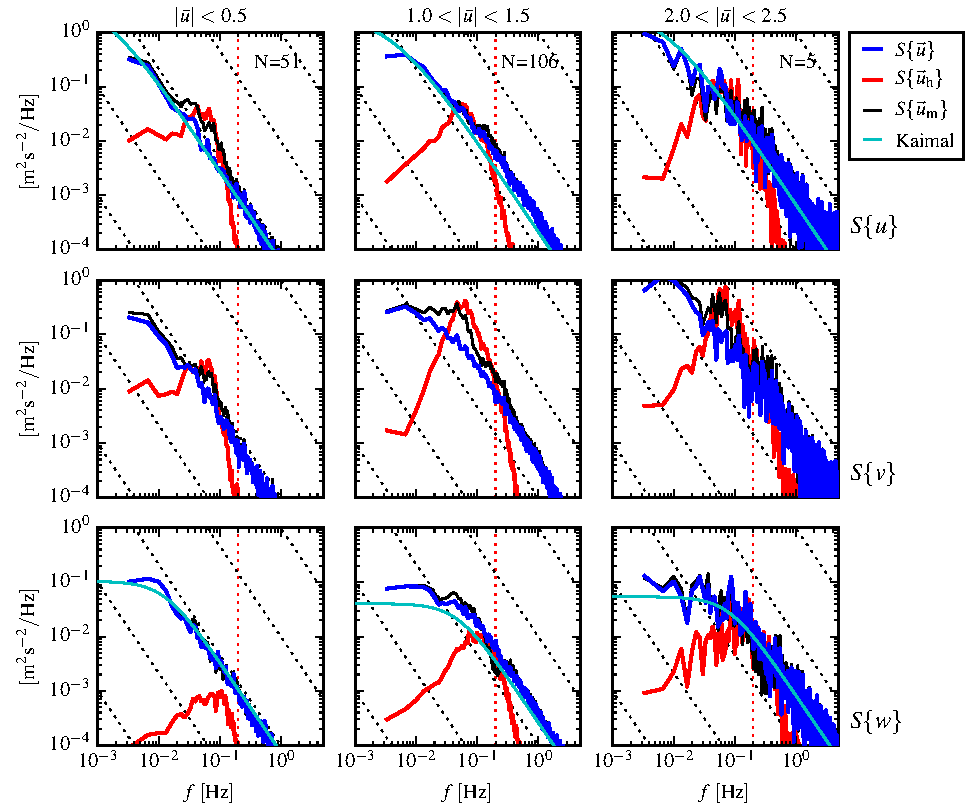
\includegraphics{SpecFig02_SMnose}
  \caption{Turbulence spectra from the StableMoor buoy. The axes-layout and annotations are identical to Figure \ref{fig:spec:ttm}.}
  \label{fig:spec:sm}
\end{figure*}

\subsection{Torpedo Spectra}

\begin{figure}[t]
  \centering
  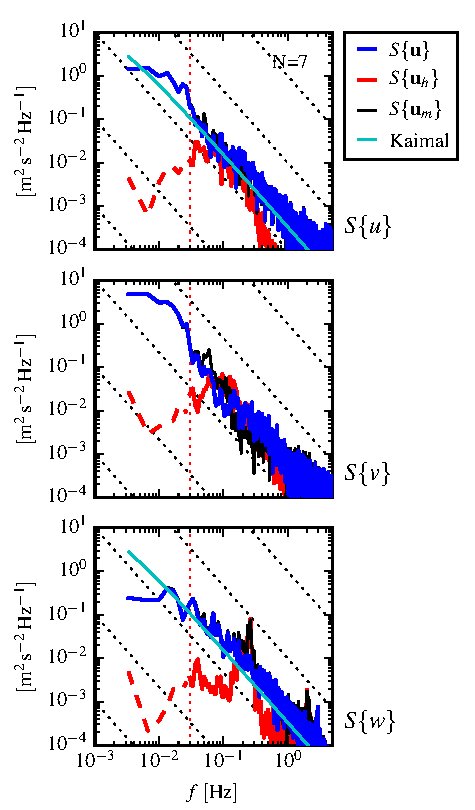
\includegraphics{SpecFig03_TTT}
  \caption{Turbulence spectra from the turbulence torpedo during a 35 minute period when the mean velocity was 1.3 m/s. Annotations and line colors are identical to Figure \ref{fig:spec:ttm}.}
  \label{fig:spec:ttt}
\end{figure}

\subsection{Reynold's stresses}

\begin{figure*}[t]
  \centering
  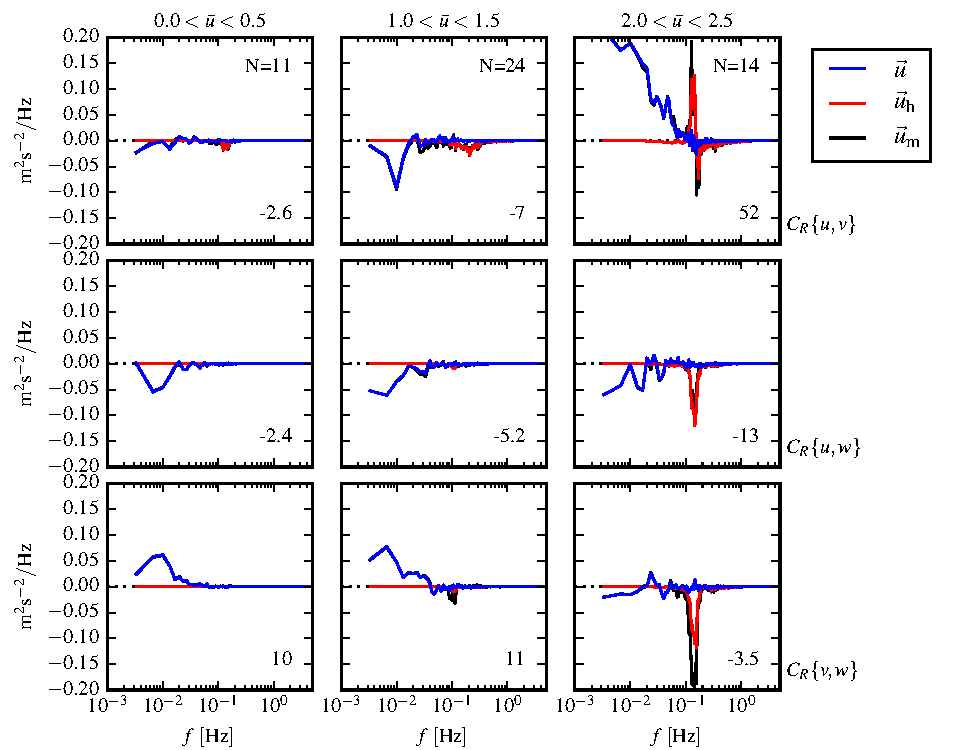
\includegraphics{StressSpec_TTM_03}
  \caption{The real part of the cross-spectral density between velocity components measured by the TTM. The upper-row is the $u$-$v$ cross-spectral density, the middle-row is the $u$-$w$ cross-spectral density, and the bottom-row is the $v$-$w$ cross-spectral density.  The columns are for different ranges of the stream-wise mean velocity magnitude. The blue line is the cross-spectrum between components of motion-corrected velocity, the red line is the cross-spectrum between components of head-motion, and the black line is the cross-spectrum between components of uncorrected velocity. N is the number of spectral ensembles in each column. The number in the lower right corner of each panel is the motion-corrected Reynold's stress (integral of the blue line) in units of 1e-4 $\mathrm{m^2s^{-2}}$.}
  \label{fig:stressspec:ttm}
\end{figure*}

\begin{figure*}[t]
  \centering
  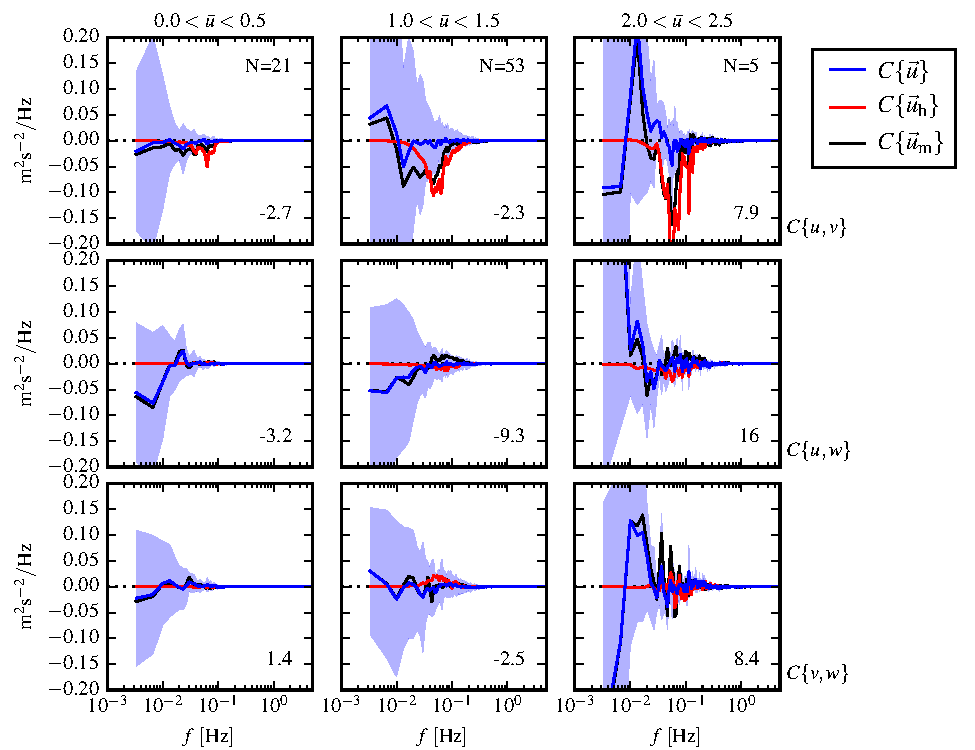
\includegraphics{StressSpec_SM_03}
  \caption{The real part of the cross-spectral density between velocity components measured by the StableMoor buoy. The axes-layout and annotations are identical to Figure \ref{fig:stressspec:ttm}.}
  \label{fig:stressspec:sm}
\end{figure*}

%\section{Other stuff}

\begin{figure*}[t]
  \centering
  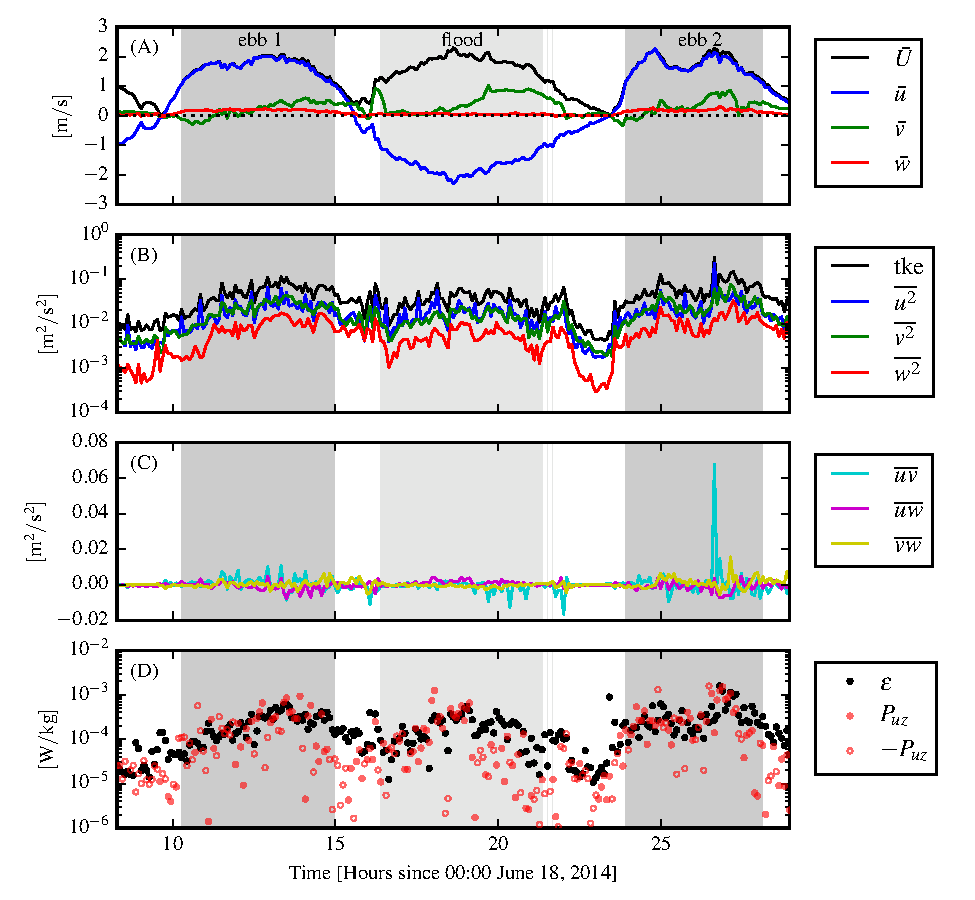
\includegraphics{TurbTime_TTM_01}
  \caption{Time-series of mean velocities (A), turbulence energy and its components (B), Reynold's stresses (C), and turbulence dissipation rate (D) measured by the TTM during the June, 2014 deployment. Shading indicates periods of ebb ($\bar{u}>0.2$, grey), and flood ($\bar{u}<-0.2$, lighter grey).}
  \label{fig:turbtime:ttm}
\end{figure*}




%%% Local Variables:
%%% mode: latex
%%% TeX-master: "Kilcher_etal_IMU-ADV"
%%% End:
